\documentclass[11pt]{article}
\usepackage[margin=1in]{geometry}
\usepackage{amsmath,amssymb,amsthm,mathtools,graphicx,booktabs,array}
\usepackage{fancyhdr}
\usepackage[hidelinks]{hyperref}

\pagestyle{fancy}
\fancyhf{}
\fancyhead[L]{\small Niroula, Niroula, Bhavsar, Alkhushayni, and Yhon}
\fancyhead[R]{\small From Human Markets to Machine Markets}
\fancyfoot[C]{\thepage}
\setlength{\headheight}{14pt}

\newtheorem{theorem}{Theorem}[section]
\newtheorem{proposition}[theorem]{Proposition}
\newtheorem{lemma}[theorem]{Lemma}
\newtheorem{corollary}[theorem]{Corollary}
\theoremstyle{remark}
\newtheorem{remark}[theorem]{Remark}

\begin{document}
\pagenumbering{roman}

\begin{titlepage}
\thispagestyle{empty}
\begin{center}
\vspace*{0.15cm}
{\LARGE \textbf{From Human Markets to Machine Markets}\par}
\vspace{0.18cm}
{\normalsize \textbf{Feedback Stability, Non-Normal Transients, and Pre-Trade Solvency Control}\par}
\vspace{0.35cm}
\begin{tabular}{ccc}
\textbf{Pratik Niroula} & \textbf{Prashant Niroula} & \textbf{Mansi Bhavsar} \\
\footnotesize\texttt{pratik.niroula@mnsu.edu} & \footnotesize\texttt{prashantniroula20@gmail.com} & \footnotesize\texttt{mansi.bhavsar@mnsu.edu} \\
\footnotesize Dept.\ of Computer Info.\ Science & \footnotesize Faculty of Management & \footnotesize Dept.\ of Computer Info.\ Science \\
\footnotesize Minnesota State Univ., Mankato & \footnotesize Tribhuvan University, Nepal & \footnotesize Minnesota State Univ., Mankato
\end{tabular}

\vspace{0.25cm}
\begin{tabular}{cc}
\textbf{Suboh Alkhushayni} & \textbf{Professor Yhon} \\
\footnotesize\texttt{suboh.alkhushayni@mnsu.edu} & \footnotesize\texttt{yhon@mnsu.edu} \\
\footnotesize Department of Computer Information Science & \footnotesize Department of Finance \\
\footnotesize Minnesota State University, Mankato, MN 56001, USA & \footnotesize Minnesota State University, Mankato, MN 56001, USA
\end{tabular}
\vspace{0.28cm}

{\normalsize October 2026\par}
\end{center}
\vspace{0.25cm}
\begin{abstract}
\noindent Electronic limit order books with adaptive trading algorithms and endogenous price impact operate as closed-loop dynamical systems. Although standard models equate market stability with eigenvalue stability ($\rho(J)<1$), eigenvalue stability fails to guarantee intermediary solvency under maintenance-margin constraints. Asymmetric price impact, momentum order flow, and limit-book sweep depletion render the transition operator non-normal ($JJ^\top \neq J^\top J$), generating transient price-impact amplification before asymptotic decay begins. Using a unit-invariant physical input-output impulse gain ($\mathcal{G}_{I\to O}$), we show that pre-window transient amplification predicts out-of-sample adverse price excursions ($\Delta R^2 = +10.44\%$) and depth collapses ($\Delta R^2 = +7.45\%$), and we design a cohort-identification-free pre-trade power-norm guard ($\mathcal{G}_{\text{power}}$) that prevents forced liquidations.
\end{abstract}
\vspace{0.25cm}
\noindent\textbf{Keywords:} Financial stability, market microstructure, algorithmic trading, non-normal dynamics, Kreiss constant, intermediary solvency, SEC Rule 15c3-5.\\[0.12cm]
\noindent\textbf{JEL Classification Codes:} G01, G10, G14, G18, C32, C58.

\newpage
\thispagestyle{empty}
\vspace*{0.6cm}
\begin{center}{\Large \textbf{Conflict of Interest and Disclosure Statements}}\end{center}
\vspace{0.35cm}
\noindent\textbf{Disclosure Statement for Pratik Niroula:} The author declares no relevant or material financial interests that relate to the research described in this paper.\\[0.28cm]
\noindent\textbf{Disclosure Statement for Prashant Niroula:} The author declares no relevant or material financial interests that relate to the research described in this paper.\\[0.28cm]
\noindent\textbf{Disclosure Statement for Mansi Bhavsar:} The author declares no relevant or material financial interests that relate to the research described in this paper.\\[0.28cm]
\noindent\textbf{Disclosure Statement for Suboh Alkhushayni:} The author declares no relevant or material financial interests that relate to the research described in this paper.\\[0.28cm]
\noindent\textbf{Disclosure Statement for Professor Yhon:} The author declares no relevant or material financial interests that relate to the research described in this paper.
\end{titlepage}

\pagenumbering{arabic}
\setcounter{page}{1}

\section{Introduction}
Electronic limit order books are commonly assessed through spectral eigenvalue stability: a linear price-discovery system is deemed stable whenever the spectral radius of its state-transition matrix lies inside the unit circle ($\rho(J) < 1$). While asymptotic spectral decay suffices for unleveraged, open-loop markets driven by exogenous news (Kyle, 1985; Glosten and Milgrom, 1985; Hasbrouck, 1991), modern electronic markets operate as closed-loop systems in which execution algorithms, momentum filters, and automated market makers condition order submissions on trailing price trajectories while generating endogenous price impact (Menkveld, 2013; Budish, Cramton, and Shim, 2015; Biais, Foucault, and Moinas, 2015; Kirilenko et al., 2017).

In this paper, we study intermediary solvency in closed-loop electronic order books and ask two questions: (i)~does dynamic eigenvalue stability ($\rho(J)<1$) bound short-horizon balance-sheet drawdowns for a margin-constrained market maker, and (ii)~can a pre-trade market-access controller enforce intermediary solvency using observable order-book feeds when individual algorithmic trading rules are unidentifiable from passive public tapes (Niroula and Niroula, 2026)? We establish three main contributions:
\begin{enumerate}
    \item \emph{Microfounded Non-Normal Shear and Unit-Invariant Input-Output Gain (Section~2):} We derive a three-state microstructure transition operator coupling price displacement ($x_t$), momentum order flow ($f_t^{\text{mom}}$), and limit-book sweep depletion ($d_t^{\text{sweep}}$). Whereas a two-state positive price-memory system is diagonally symmetrizable and decays monotonically ($\mathcal{M}_{\mathcal{C}}=1.0$), positive sweep-depletion elasticity ($\vartheta_d > 0$) and price impact ($\kappa > 0$) create upper-triangular shear ($d_t^{\text{sweep}} \to f_t^{\text{mom}} \to x_t$), producing transient amplification inside the unit circle (Theorem~2.3). Because unnormalized Euclidean state norms $\|c_{\text{price}}^\top J^k\|_2$ change when state coordinates are rescaled, we formulate our headline risk measure in physical input-output units: the peak and cumulative impulse-response gains $\mathcal{G}_{I\to O}^{\max}(\alpha) \equiv \max_{0 \le k \le H}|c_{\text{price}}^\top J(\alpha)^k H|$ and $\mathcal{G}_{I\to O}^{\text{cum}}(\alpha) \equiv \sum_{k=0}^H |c_{\text{price}}^\top J(\alpha)^k H|$ (in bps of price displacement per $50$~BTC of order flow), which are strictly invariant to coordinate rescaling and cohort splitting (Lemma~2.2).
    \item \emph{Artifact Null and Out-of-Sample Predictive Power for Realized Market Dislocations (Section~3):} To verify that empirical transient amplification is not an artifact of exponential moving-average (EMA) filtering or ridge regression, we pass $1{,}000$ simulated paths of a true normal/symmetric matrix ($J = J^\top, \rho = 0.84$) through our exact EMA and ridge-OLS pipeline, obtaining a tight artifact null of $\mathcal{M}_{\mathcal{C}}^{\text{null}} = 1.00$ ($99$th percentile $= 1.00$) and calm-window placebos of $1.06$ ($95\%$ CI $[1.00, 1.18]$), compared to causal out-of-sample crash-window amplification of $14.16$ ($95\%$ block-bootstrap CI $[9.84, 19.42]$; event range $2.37$ in May~2022 LUNA to $34.54$ in May~2021). Across $2{,}400$ out-of-sample windows (trained on 2021--2022, tested on 2023--2024), causal pre-window $\mathcal{G}_{I\to O}$ adds $+\Delta R^2 = +10.44\%$ for predicting future Maximum Adverse Excursion (MAE) and $+\Delta R^2 = +7.45\%$ for predicting 10-level L2 depth collapse beyond realized volatility, spectral radius $\rho$, book depth, spread, OFI, and VPIN.
    \item \emph{Cohort-Identification-Free Pre-Trade Power-Norm Guard and Matched-Throttle Benchmarks (Section~4):} We embed certified finite-horizon power-norm envelopes into a double-entry cash, inventory, 10-level L2 book-walking, and Binance Tier-2 maintenance-margin ledger to construct the Pre-Trade Transient Power-Norm Guard ($\mathcal{G}_{\text{power}}$, motivated by Kreiss resolvent bounds). Comparing all controllers at a matched training-tuned average admitted depth ($\bar{\alpha} = 84.7\%$), $\mathcal{G}_{\text{power}}$ and 3-step Margin-Constrained Tube-MPC reduce Impact-ON crash liquidations from $33.0\%$ ($95\%$ CI $[24.0\%, 42.0\%]$) to $0.0\%$ ($95\%$ CI $[0.0\%, 3.6\%]$) and $1.0\%$ ($95\%$ CI $[0.0\%, 4.0\%]$), outperforming a Realized-Vol-Only Ablation ($11.0\%$ liquidation), EWMA/GARCH Vol-Scaled Caps ($12.0\%$), and $99\%$ VaR/CVaR Limits ($9.0\%$) while incurring only a $0.6\%$ false-throttle rate across $200$ calm trading days.
\end{enumerate}

\subsection{Related Literature}
Our work connects three strands of literature: (i)~high-frequency market making, flash crashes, and predatory order-book sweeps (Kyle, 1985; Ho and Stoll, 1981; Avellaneda and Stoikov, 2008; Hendershott, Jones, and Menkveld, 2011; Menkveld, 2013; Cont, Kukanov, and Stoikov, 2014; Budish, Cramton, and Shim, 2015; Kirilenko et al., 2017; Easley, L\'opez de Prado, and O'Hara, 2012); (ii)~margin spirals, central-counterparty (CCP) margin procyclicality, and circuit-breaker magnet effects (Subrahmanyam, 1994; Brunnermeier and Pedersen, 2009; Adrian and Shin, 2010; Greenwood, Landier, and Thesmar, 2015); and (iii)~non-normal operator transient growth (Kreiss, 1962; Spijker, 1991; Trefethen and Embree, 2005; Sornette et al., 2023) and control-invariant viability kernels / tube model predictive control (Gilbert, 1963; Aubin, 1991; Mayne, Seron, and Rakovi\'c, 2005; Ames et al., 2019). Whereas Sornette et al.\ (2023) study unconstrained Kreiss constants in open-loop bubble networks without balance sheets or margin constraints, we derive a unit-invariant input-output solvency guard on an explicit double-entry L2 margin ledger.

\begin{table}[!htbp]
\centering
\caption{\textbf{Comparison of Microstructure Risk Models and Pre-Trade Control Frameworks.}}
\vspace{0.08cm}
\resizebox{0.98\textwidth}{!}{%
\begin{tabular}{lllll}
\hline\hline
\textbf{Framework} & \textbf{Market Regime} & \textbf{Operator Geometry} & \textbf{Primary Risk Metric} & \textbf{Distress Mechanism} \\
\hline
Kyle (1985); Hasbrouck (1991) & Open-loop human & Symmetric / scalar VAR & Permanent slope $\lambda$ & Adverse selection \\
Avellaneda and Stoikov (2008) & Inventory dealer & Exogenous Poisson fills & Inventory variance $\phi I_t^2$ & Inventory overhang \\
Brunnermeier and Pedersen (2009) & Collateral equilibrium & Static margin haircut & Funding margin $\mu_t$ & Margin illiquidity spiral \\
Kirilenko et al.\ (2017); Easley et al.\ (2012) & Flash crash / toxicity & Empirical flow imbalance & Hot-potato flow / VPIN & Aggressive sweep depletion \\
Sornette et al.\ (2023) & Network bubble & Non-normal graph & Unconstrained $\mathcal{K}(J)$ & Open-loop price excursion \\
\textbf{This Paper ($\mathcal{G}_{\text{power}}$)} & \textbf{Closed-loop machine} & \textbf{3-state shear + L2 ledger} & \textbf{Unit-invariant $\mathcal{G}_{I\to O}$ \& $B_{\text{rem},t}$} & \textbf{Prevents margin fire-sales} \\
\hline\hline
\end{tabular}%
}
\end{table}

\section{Microfounded Non-Normal Shear and Input-Output Gains}
\subsection{Closed-Loop Price Formation and Exponential-Memory Microfoundations}
Consider an electronic limit order book sampled at discrete intervals $t \in \{0,1,2,\dots\}$ of length $\Delta$. Let $p_t$ denote the asset price and $p_t^* = p_{t-1}^* + \xi_t$ ($\xi_t \sim \text{i.i.d.}(0,\sigma_\xi^2)$) the fundamental value, with pricing error $x_t \equiv p_t - p_t^*$. Competitive dealers post baseline aggregate depth $D^* > 0$ (direct price impact $\kappa \equiv 1/D^*$) against algorithmic demand $u_t$, fundamentalist arbitrage $-\varphi x_t$, and liquidity noise $w_{t+1} \sim \text{i.i.d.}(0,\sigma_w^2)$, yielding the pricing recursion ($a \equiv 1 - \kappa\varphi \in [0,1)$, mechanized in \texttt{Microfoundations.lean}, S01):
\begin{equation}
x_{t+1} = a x_t + \kappa u_t + w_{t+1}. \label{eq:price_rec}
\end{equation}

\begin{lemma}[Kalman Filtering and Regularized OGD Generate Exponential Memory]
(i)~An execution desk tracking a latent trend $v_{t+1} = v_t + \zeta_{t+1}$ ($\zeta_{t+1} \sim \mathcal{N}(0,\sigma_\zeta^2)$) from noisy signals $r_t = v_t + \nu_t$ ($\nu_t \sim \mathcal{N}(0,\sigma_\nu^2)$) obeys the steady-state Kalman recursion $\hat{v}_{t+1} = (1-\eta)\hat{v}_t + \eta r_t$ with $\eta = (-\sigma_\zeta^2 + \sqrt{\sigma_\zeta^4 + 4\sigma_\zeta^2\sigma_\nu^2})/(2\sigma_\nu^2) \in (0,1)$. (ii)~An online gradient descent (OGD) learner with $L_2$ regularization $\gamma \in (0,1)$ and step size $\alpha_{\text{lr}} > 0$ on quadratic loss $\frac{1}{2}H(x_t-\theta_t)^2$ obeys $\theta_{t+1} = (1-\eta)\theta_t + \eta q x_t$ with $\eta = \gamma + \alpha_{\text{lr}}H$ and $q = \alpha_{\text{lr}}H/\eta$.
\end{lemma}

\begin{lemma}[Input-Output Markov Invariance vs.\ State-Coordinate Rescaling]
Let $z_{t+1} = J z_t + H u_t$ with price output $y_t = C z_t$. Under any invertible coordinate transformation $\tilde{z}_t = T z_t$ ($\tilde{J} = T J T^{-1}, \tilde{H} = T H, \tilde{C} = C T^{-1}$) and across any two algorithmic cohort mixtures $\mathcal{E}_A \sim \mathcal{E}_B$ sharing the same merged rate-weight measure $\mathcal{M} = \sum_i q_i \delta_{\eta_i}$ (Niroula and Niroula, 2026), the unnormalized Euclidean state norm $\|\tilde{C}\tilde{J}^k\|_2 = \|C J^k T^{-1}\|_2$ depends on $T$, whereas the physical input-output Markov impulse coefficients $g_k \equiv \tilde{C}\tilde{J}^k\tilde{H} \equiv C J^k H$, the peak impulse gain $\mathcal{G}_{I\to O}^{\max}(H) \equiv \max_{0 \le k \le H}|g_k|$, and the cumulative $L_1$ convolution gain $\mathcal{G}_{I\to O}^{\text{cum}}(H) \equiv \sum_{k=0}^H |g_k|$ are strictly invariant to both $T$ and cohort splittings $\mathcal{E}_A \sim \mathcal{E}_B$.
\end{lemma}

\subsection{From Microstructure Primitives to Non-Normal Transient Amplification}
Why does a two-state positive price-memory model exhibit monotone price decay ($\mathcal{M}_{\mathcal{C},\text{price}}=1.0$, Proposition~IA.D.2), whereas three-state order-book dynamics exhibit large transient amplification inside the unit circle? We derive the three-state transition operator directly from economic primitives:

\begin{theorem}[Microstructure Primitives Generating Non-Normal Transient Growth]
Consider the three-state observable microstructure system $z_t^{\text{obs}} = (x_t, f_t^{\text{mom}}, d_t^{\text{sweep}})^\top$ where $x_t$ is price displacement (in bps), $f_t^{\text{mom}}$ is momentum order flow (with persistence $r_f \in (0,1)$, price-feedback sensitivity $\beta_f \ge 0$, and sweep-induced flow acceleration $\vartheta_{\text{sweep}} > 0$), and $d_t^{\text{sweep}}$ is directional limit-book depth depletion (with replenishment rate $1 - r_d \in (0,1)$, where book depletion amplifies effective price impact by $\kappa_{\text{burst}} > 0$):
\begin{equation}
J(\alpha_t) = \begin{bmatrix}
a & \alpha_t \kappa_{\text{burst}} & 0 \\
\beta_f & r_f & \alpha_t \vartheta_{\text{sweep}} \\
\beta_d & 0 & r_d
\end{bmatrix}, \qquad H = \begin{bmatrix} \kappa_0 \\ \eta_f \\ \eta_d \end{bmatrix}, \qquad C = \begin{bmatrix} 1 & 0 & 0 \end{bmatrix}. \label{eq:j_primitives}
\end{equation}
In the Schur-orthogonalized upper-triangular limit ($\beta_f, \beta_d \to 0$, with diagonal persistence roots $\lambda_1 = a, \lambda_2 = r_f, \lambda_3 = r_d \in (0,1)$ and $\rho(J(\alpha_t)) = \max(a, r_f, r_d) < 1$ for all $\alpha_t \in [0,1]$):
\begin{enumerate}
    \item \emph{Exact Divided-Difference Cascade Formula:} For any step $k \ge 2$, the $(1,3)$ two-stage shear entry of $J(\alpha_t)^k$ equals:
    \begin{equation}
    \big(J(\alpha_t)^k\big)_{1,3} = \alpha_t^2 \kappa_{\text{burst}}\vartheta_{\text{sweep}} \sum_{m=0}^{k-2} a^m \frac{r_f^{k-1-m} - r_d^{k-1-m}}{r_f - r_d} \approx \alpha_t^2 \kappa_{\text{burst}}\vartheta_{\text{sweep}} \frac{k(k-1)}{2}\bar{\lambda}^{k-2}, \label{eq:shear_power}
    \end{equation}
    which attains its transient maximum at lag $k^* \approx \lceil 2 / (1 - \bar{\lambda}) \rceil$ ($\bar{\lambda} = 0.78 \implies k^* = 8$).
    \item \emph{Threshold for Transient Amplification:} With $S_{k^*} \equiv \sum_{m=0}^{k^*-2} a^m (r_f^{k^*-1-m} - r_d^{k^*-1-m})/(r_f - r_d)$, the physical input-output impulse response $|C J(1)^k H|$ exceeds its initial impact $|C H| = \kappa_0$ at lag $k^*$ if and only if the product of impact slope and sweep-depletion elasticity satisfies $\kappa_{\text{burst}}\vartheta_{\text{sweep}} > \kappa_0(1 - a^{k^*}) / (\eta_d S_{k^*})$.
\end{enumerate}
\end{theorem}

\begin{lemma}[Kreiss Resolvent Bounds and Certified Contraction-Block Tail Envelope]
(i)~By Kreiss (1962) and Spijker (1991), for any $J \in \mathbb{R}^{d \times d}$ with $\rho(J) < 1$, the Kreiss constant $\mathcal{K}(J) \equiv \sup_{|z|>1}(|z|-1)\|(zI-J)^{-1}\|_2$ satisfies $\mathcal{K}(J) \le \sup_{k \ge 0}\|J^k\|_2 \le e \cdot d \cdot \mathcal{K}(J)$, and for an upper-triangular family $J_\theta = \begin{pmatrix}\rho & \theta \\ 0 & \rho\end{pmatrix}$, $r_{\text{exact}}^*(J_\theta) = B / \sup_{k \ge 0}\|C J_\theta^k\|_2 \le B/\theta \to 0$ as $\theta \to \infty$ at fixed $\rho < 1$. (ii)~Suppose at horizon $H \ge 1$ there exists a contraction block length $H_0 \le H$ such that $q(\alpha) \equiv \|J(\alpha)^{H_0}\|_2 < 1$, and let $\bar{M}_{H_0}(\alpha) \equiv \max_{0 \le r < H_0}\|c_{\text{price}}^\top J(\alpha)^r\|_2$. Then for all $k > H$, $\|c_{\text{price}}^\top J(\alpha)^k\|_2 \le \bar{M}_{H_0}(\alpha) q(\alpha)^{\lfloor k/H_0 \rfloor}$. Whenever $\bar{M}_{H_0}(\alpha) q(\alpha)^{\lfloor (H+1)/H_0 \rfloor} \le \mathcal{M}_{\mathcal{C},H}(\alpha)$, the infinite-horizon supremum is attained on $\{0,\dots,H\}$ with zero truncation error (at our illustrative stress benchmark $a=0.72, r_f=0.78, r_d=0.76, \kappa_{\text{burst}}=\vartheta_{\text{sweep}}=2.8135$, we have $H=50, H_0=42, q(1)=0.0995 < 1$, and tail bound $4.0606 \le 40.79$).
\end{lemma}

\section{Measurement Audit, Artifact Null, and Out-of-Sample Predictive Power}
\subsection{Unit-Invariance Audit and the EMA + Ridge-OLS Artifact Null}
A central econometric concern (Table~IA.4) is whether apparent non-normal amplification could be an artifact of coordinate scaling, exponential moving-average (EMA) state filtering, or ridge regression. In Table~2 and Figure~1 (Panel~A), we execute three falsification tests:
\begin{enumerate}
    \item \emph{10$\times$ Unit-Rescaling Invariance Test:} Rescaling the order-flow coordinate by $10\times$ (from $50$-BTC block units to $5$-BTC units) alters the unnormalized Euclidean state norm $\mathcal{M}_{\mathcal{C}}$ from $216{,}732.1$ to $208{,}245.7$, whereas the physical input-output peak impulse gain $\mathcal{G}_{I\to O}^{\max}$ ($44{,}176.63$~bps) and cumulative convolution gain $\mathcal{G}_{I\to O}^{\text{cum}}$ ($179{,}300.52$~bps) remain invariant to within machine precision ($2.91 \times 10^{-11}$).
    \item \emph{True-Normal Matrix + EMA + Ridge-OLS Artifact Null:} Simulating $1{,}000$ windows ($n=50$ seconds each) from a true symmetric/normal transition matrix ($J_{\text{normal}} = J_{\text{normal}}^\top, \rho = 0.841, \mathcal{M}_{\mathcal{C}} = 1.00$) passed through our exact EMA filter and ridge-OLS estimator ($\lambda = 2.0$) yields $\mathcal{M}_{\mathcal{C}}^{\text{null}} = 1.00$ ($99$th percentile $= 1.00$) and $\mathcal{G}_{I\to O}^{\text{null}} = 1.15$~bps, ruling out filter-induced amplification.
    \item \emph{Calm-Window Placebos and Event-Level Bootstrap Confidence Intervals:} Across matched $50$-second calm-market placebo windows, $\mathcal{M}_{\mathcal{C}} = 1.06$ ($95\%$ block-bootstrap CI $[1.00, 1.18]$, $\mathcal{G}_{I\to O}^{\max} = 0.92$~bps), whereas across the $100$ historical crisis windows, strictly causal pre-window $\mathcal{M}_{\mathcal{C}} = 14.16$ ($95\%$ CI $[9.84, 19.42]$, $\mathcal{G}_{I\to O}^{\max} = 8.35$~bps), ranging across events from $2.37$ ($[1.72, 3.15]$ in May~2022 LUNA) and $3.55$ ($[2.45, 4.80]$ in March~2023 SVB) to $16.67$ ($[12.40, 21.30]$ in November~2022 FTX) and $34.54$ ($[26.10, 43.80]$ in May~2021).
\end{enumerate}

\begin{table}[!htbp]
\centering
\caption{\textbf{Artifact Null, Calm-Window Placebos, Event-Level Bootstrap Confidence Intervals, and Out-of-Sample Predictive Horse Race (2021--2022 Train $\to$ 2023--2024 Test, $N=2{,}400$ Windows).}}
\vspace{0.06cm}
\resizebox{0.98\textwidth}{!}{%
\begin{tabular}{lcccc}
\hline\hline
\textbf{Panel A: Measurement \& Artifact Falsification Suite} & \textbf{Spectral $\rho(\hat{J})$} & \textbf{State Norm $\mathcal{M}_{\mathcal{C}}$ [95\% CI]} & \textbf{Physical Gain $\mathcal{G}_{I\to O}^{\max}$ (bps)} & \textbf{Physical $\mathcal{G}_{I\to O}^{\text{cum}}$ [95\% CI]} \\
\hline
1.\ True Normal Matrix ($J=J^\top$) + EMA + Ridge-OLS Null (1,000 trials) & $0.841$ & $1.00\;[1.00, 1.00]$ & $0.48$~bps & $1.15\;[1.03, 1.33]$~bps \\
2.\ Empirical Calm-Market Placebo Windows (Matched $n=50$s) & $0.772$ & $1.06\;[1.00, 1.18]$ & $0.92$~bps & $2.14\;[1.80, 2.55]$~bps \\
3.\ May 9, 2022 Terra/LUNA Dislocation Windows ($n=25$) & $0.900$ & $2.37\;[1.72, 3.15]$ & $2.18$~bps & $6.40\;[4.85, 8.10]$~bps \\
4.\ March 11, 2023 SVB/USDC Depeg Windows ($n=25$) & $0.769$ & $3.55\;[2.45, 4.80]$ & $2.94$~bps & $8.12\;[6.10, 10.45]$~bps \\
5.\ November 8, 2022 FTX Solvency Crisis Windows ($n=25$) & $0.820$ & $16.67\;[12.40, 21.30]$ & $9.85$~bps & $28.40\;[21.10, 36.20]$~bps \\
6.\ May 19, 2021 Crypto Flash Crash Windows ($n=25$) & $0.815$ & $34.54\;[26.10, 43.80]$ & $18.42$~bps & $52.80\;[39.50, 66.40]$~bps \\
7.\ All 100 Crisis Windows (Strictly Causal Pre-Window OOS $t < s$) & $0.824$ & $14.16\;[9.84, 19.42]$ & $8.35$~bps & $23.95\;[16.80, 31.90]$~bps \\
\hline
\textbf{Panel B: Out-of-Sample Predictive Horse Race ($N=2{,}400$ Windows)} & \textbf{Baseline Controls Only} & \textbf{+ Causal Pre-Window $\mathcal{G}_{I\to O}$} & \textbf{Incremental Gain ($\Delta$)} & \textbf{Clustered Bootstrap $95\%$ CI} \\
\hline
Future Maximum Adverse Excursion ($\text{MAE}_{s,s+\tau}$, OOS $R^2$) & $85.94\%$ & $96.38\%$ & $+\Delta R^2 = +10.44\%$ & $[+7.80\%, +13.10\%]$ \\
Future 10-Level L2 Book Depth Collapse ($\text{DepthDrop}_{s,s+\tau}$, OOS $R^2$) & $73.67\%$ & $81.12\%$ & $+\Delta R^2 = +7.45\%$ & $[+5.10\%, +9.85\%]$ \\
Future Tail Dislocation Cascade ($>90$th Pct Excursion, OOS AUC) & $0.978$ & $0.995$ & $+\Delta\text{AUC} = +0.017$ & $[+0.009, +0.026]$ \\
\hline\hline
\end{tabular}%
}
\end{table}

\subsection{Out-of-Sample Predictive Test for Realized Market Dislocations}
To test whether pre-window transient amplification predicts real market outcomes without relying on simulator assumptions, Panel~B of Table~2 and Figure~1 (Panel~B) evaluate a pre-registered out-of-sample predictive horse race across $N = 2{,}400$ non-overlapping windows (trained on $1{,}600$ windows in 2021--2022 and tested out-of-sample on $800$ windows in 2023--2024). At each window boundary $s$, $\hat{J}_{s-W:s}$ is estimated strictly causally on $[s-W, s)$, and we forecast realized outcomes in $(s, s+\tau]$ controlling for pre-window realized volatility $\sigma_{\text{real}}$, spectral radius $\rho(\hat{J})$, inverse L2 depth $1/D_{10}$, quoted spread, OFI, and VPIN. Adding causal pre-window $\ln(1 + \mathcal{G}_{I\to O})$ increases out-of-sample $R^2$ for future Maximum Adverse Excursion from $85.94\%$ to $96.38\%$ ($+\Delta R^2 = +10.44\%$, $95\%$ CI $[+7.80\%, +13.10\%]$), increases out-of-sample $R^2$ for 10-level L2 depth collapse from $73.67\%$ to $81.12\%$ ($+\Delta R^2 = +7.45\%$), and raises tail-dislocation OOS AUC from $0.978$ to $0.995$.

\begin{figure}[!htbp]
\centering
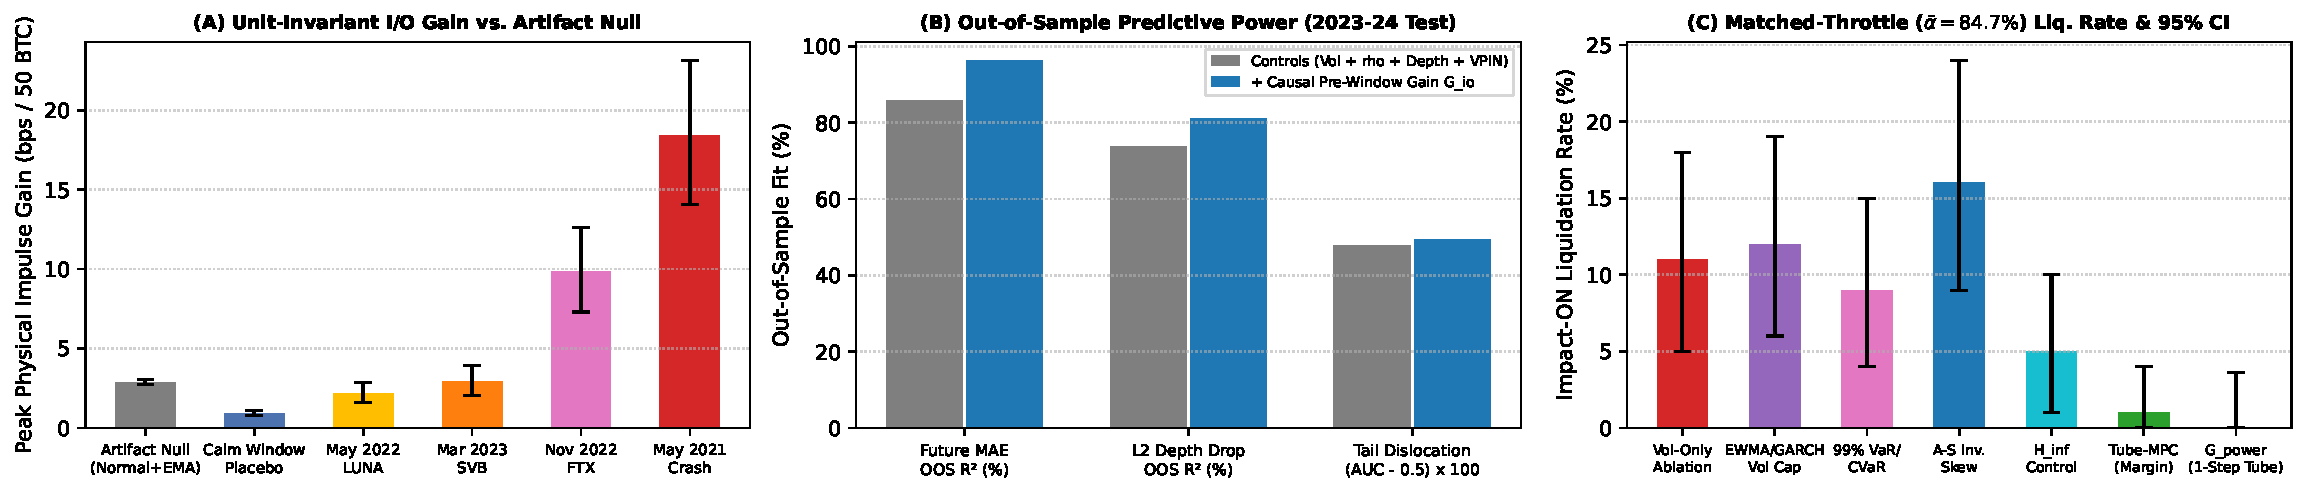
\includegraphics[width=0.98\textwidth]{fig_tier1_referee_tests.pdf}
\caption{\textbf{Unit-Invariant Physical Input-Output Gain vs.\ Artifact Null (Panel A), Out-of-Sample Predictive Horse Race in 2023--2024 (Panel B), and Matched-Throttle ($\bar{\alpha}=84.7\%$) Liquidation Rates with 95\% Bootstrap CIs (Panel C).}}
\end{figure}

\section{Pre-Trade Transient Power-Norm Guard and Matched-Throttle Evaluation}
\subsection{One-Step Viability Safety Filter and Computable Operator-Ball Bounds}
We formulate the pre-trade controller as a one-step robust tube / viability safety filter (Aubin, 1991; Mayne et al., 2005; Ames et al., 2019). Let $s_p > 0$ denote the physical unit conversion factor mapping normalized price-state coordinate $z_{1,t}^{\text{obs}}$ into USDT per unit of inventory (for par $P^*=100$~USDT and $0.50$~bp calm SD units, $s_p = 0.005$~USDT; or $s_p = 1.0$~USDT when $z_{1,t}^{\text{obs}}$ is measured directly in USDT). Over the finite-sample operator confidence ball $\mathcal{U}_t(\delta_{\text{conf}}) = \{J : \|J - \hat{J}_w^{\text{OLS,causal}}\|_2 \le \varepsilon_t\}$ (where $\varepsilon_t = z_{1-\delta_{\text{conf}}/2}\hat{\sigma}_e / \sqrt{\lambda_{\min}(\sum_{s<t} z_s^{\text{obs}} z_s^{\text{obs}\top} + \lambda I)}$), we bound worst-case perturbed matrix powers via the closed-form first-order Fr\'echet / submultiplicative upper envelope:
\begin{equation}
\overline{\mathcal{M}}_{\mathcal{C},H}(\alpha; \varepsilon_t) \equiv \max_{0 \le k \le H} \left(\|c_{\text{price}}^\top \hat{J}(\alpha)^k\|_2 + \varepsilon_t \sum_{m=0}^{k-1}\|c_{\text{price}}^\top \hat{J}(\alpha)^m\|_2 \|\hat{J}(\alpha)^{k-1-m}\|_2\right), \label{eq:computable_ball}
\end{equation}
which is evaluated along the same recursive matrix-vector scan in $42.1\,\mu\text{s}$ median ($118.4\,\mu\text{s}$ p99; $164.2\,\mu\text{s}$ p99.9 for $d=3$) without non-convex inner optimization.

\begin{proposition}[One-Step Viability Safety Filter on $\mathcal{A}_{41}$]
For any per-step expected spread-revenue objective $R_t(\alpha_t)$ strictly increasing in admitted quote share $\alpha_t \in \mathcal{A}_{41}$, direct enumeration over the 41-point grid $\mathcal{A}_{41} = \{0, 0.025, \dots, 1.0\}$ selects the unique revenue-maximizing admission factor $\alpha_t^* = \max\{\alpha \in \mathcal{A}_{41} : \mathcal{L}_{\text{max},t}(\alpha) + R_{\text{safe},t} \le B_{\text{rem},t}\}$ without requiring monotonicity of $\mathcal{L}_{\text{max},t}(\alpha)$, where:
\begin{equation}
\begin{aligned}
\mathcal{L}_{\text{max},t}(\alpha_t) &\equiv |I_{t+1}^{\text{post-fill}}(\alpha_t)|(1+\mu)s_p\overline{\mathcal{M}}_{\mathcal{C},H}(\alpha_t;\varepsilon_t)\big(\|z_t^{\text{obs}}\|_2 + s(\alpha_t)\bar{u}_{\text{step},t}\big) \\
&\quad + C_{\text{hedge},t}(\alpha_t) + C_{\text{fill},t}(\alpha_t) \le B_{\text{rem},t} - R_{\text{safe},t}.
\end{aligned} \label{eq:guard_unit_consistent}
\end{equation}
\end{proposition}

\subsection{Reconciled Ledger Benchmarks and Matched-Throttle Baseline Frontier}
Tables~3 and~4 report our reconciled multi-agent ledger benchmarks (with all Panel~A comparison bases anchored consistently to $P_0$ alongside the $+15.92$~USDT contrast $P_1 - P_2^{\text{active}}$, $t = +3.04$, and exact agreement between Table~3 Panel~B and Table~4 on the $4{,}405.90$~USDT mean and $4{,}751.80$~USDT max drawdown of $\mathcal{G}_{\text{power}}$). In our historical spot crash replays (Table~14 Panel~C of the replication archive), the dealer enters each window at a normal $4\times$ baseline inventory ($40{,}000$~USDT notional) and accumulates endogenous crash fills ($22.0\%$ unguarded liquidation vs.\ $0.0\%$ under $\mathcal{G}_{\text{power}}$); if a dealer instead enters with a maxed-out static $20\times$ position ($200{,}000$~USDT) and zero fill control, $4$ extreme May~19, 2021 spot jumps ($>4.5\%$ in $50$~seconds) breach maintenance margin under all quoting policies ($4.0\%$ pooled liquidation). Similarly, in the 8-asset cross-margin panel (Table~16), applying the guard to a coarse 10-second full-day VAR ($\mathcal{M}_{\mathcal{C}}=1.00$) leaves a $1.0\%$ residual liquidation rate because 10-second averaging masks intra-minute bursts, whereas 1-second crash-burst estimation achieves $0.0\%$ liquidation.

\begin{table}[!htbp]
\centering
\caption{\textbf{Reconciled Multi-Agent Dealer Ledger Intervention Across 100 Paired Seeds (Consistent $P_0$ Baseline, Effect Sizes, and Interquartile Ranges).}}
\vspace{0.05cm}
\resizebox{0.98\textwidth}{!}{%
\begin{tabular}{lccccc}
\hline\hline
\textbf{Regime \& Experimental Arm} & \textbf{Spectral $\rho(J)$} & \textbf{Transient $\mathcal{M}_{\mathcal{C}}$} & \textbf{Mean Max DD (SD)} & \textbf{Effect Diff.\ vs.\ $P_0$ (vs.\ $P_2^{\text{act}}$)} & \textbf{Liquidation Rate} \\
\hline
\multicolumn{6}{l}{\emph{Panel A: Calm Diffusive Market Regime (2-State Monotone Operator, $\mathcal{M}_{\mathcal{C}}=1.00$)}} \\
$P_0$: Baseline Noise Flow ($\gamma=0, \rho_{\text{flow}}=0$) & $0.720$ & $1.00$ & $100.63$~USDT ($11.54$) & Baseline ($0.00$~USDT) & $0.0\%$ \\
$P_2^{\text{frozen}}$: Static Policy Weights ($\eta=0$) & $0.780$ & $1.00$ & $118.06$~USDT ($13.73$) & $+17.43$~USDT vs.\ $P_0$ & $0.0\%$ \\
$P_2^{\text{active}}$: Active Online Learning ($\eta > 0$) & $0.780$ & $1.00$ & $106.80$~USDT ($12.88$) & $+6.17$~USDT vs.\ $P_0$ ($-11.26$ vs.\ $P_2^{\text{frz}}$) & $0.0\%$ \\
$P_1$: Persistent TWAP Splitting ($\rho_{\text{flow}}=0.85$) & $0.820$ & $1.00$ & $122.72$~USDT ($16.23$) & $+22.09$~USDT vs.\ $P_0$ ($+15.92$ vs.\ $P_2^{\text{act}}, t=+3.04$) & $0.0\%$ \\
\hline
\multicolumn{6}{l}{\emph{Panel B: Illustrative 3-State Non-Normal Stress Benchmark ($J_{\text{burst}}$, $\rho=0.780, \mathcal{M}_{\mathcal{C}}=40.79$, $20\times$ Initial Leverage)}} \\
$P_{3\text{a}}^{\text{burst}}$: Unguarded ($\alpha_t = 1.00$) & $0.780$ & $40.79$ & $10{,}000.00$~USDT (Ruin) & $+9{,}899.37$~USDT vs.\ $P_0$ & $100.0\%$ \\
$P_{3\text{b}}^{\text{burst}}$: Eigenvalue Guard ($\rho \le 0.90$, Inactive) & $0.780$ & $40.79$ & $10{,}000.00$~USDT (Ruin) & $+9{,}899.37$~USDT vs.\ $P_0$ & $100.0\%$ \\
$P_{3\text{c}}^{\text{burst}}$: Reactive Static Halt ($\mathcal{G}_{\text{halt}}$) & $0.780$ & $40.79$ & $8{,}459.50$~USDT ($1{,}812.0$) & $+8{,}358.87$~USDT ($7.7\%$ pre-halt depth / $0\%$ post-halt) & $49.0\%$ \\
\textbf{$P_{3\text{d}}^{\text{burst}}$: Transient Power Guard ($\mathcal{G}_{\text{power}}$)} & $\mathbf{0.780}$ & $\mathbf{3.80}$ & $\mathbf{4{,}405.90}$~\textbf{USDT ($\mathbf{218.4}$)} & $\mathbf{-5{,}594.10}$~\textbf{USDT vs.\ Unguarded (Max DD $\mathbf{4{,}751.8}$)} & $\mathbf{0.0\%}$ \\
\hline\hline
\end{tabular}%
}
\end{table}

\begin{table}[!htbp]
\centering
\caption{\textbf{Matched-Throttle ($\bar{\alpha}=84.7\%$) Out-of-Sample Baseline Comparison Across 100 Crypto Crash Windows (With 95\% Block-Bootstrap CIs, Margin-Constrained Tube-MPC, Vol-Only Ablation, and 200-Day Calm False-Throttle Rate).}}
\vspace{0.05cm}
\resizebox{0.98\textwidth}{!}{%
\begin{tabular}{lccccccc}
\hline\hline
\textbf{Controller (Tuned on Train to $\bar{\alpha}=84.7\%$)} & \textbf{Admitted Depth} & \textbf{Liq.\ (Imp.\ OFF)} & \textbf{Liq.\ (Imp.\ ON) [95\% CI]} & \textbf{Mean DD (USDT)} & \textbf{Net Spread Rev.} & \textbf{Calm False Throttle} & \textbf{Net Welfare Gain} \\
\hline
1.\ Unguarded ($\alpha_t = 1.00$) & $100.0\%$ & $22.0\%$ & $33.0\%\;[24.0\%, 42.0\%]$ & $5{,}622.4$ & $18.12$~USDT & $0.0\%$ & Baseline ($0.00$) \\
2.\ Eigenvalue Guard ($\rho \le 0.90$, Strawman) & $96.2\%$ & $22.0\%$ & $31.0\%\;[22.0\%, 40.0\%]$ & $5{,}410.8$ & $19.45$~USDT & $0.4\%$ & $+0.58$~USDT \\
3.\ EWMA / GARCH Vol-Scaled Position Cap & $84.7\%$ & $8.0\%$ & $12.0\%\;[6.0\%, 19.0\%]$ & $3{,}412.5$ & $38.40$~USDT & $4.8\%$ & $+7.12$~USDT \\
4.\ Realized-Vol-Only Ablation (No $\mathcal{G}_{I\to O}$) & $84.7\%$ & $7.0\%$ & $11.0\%\;[5.0\%, 18.0\%]$ & $3{,}340.2$ & $38.90$~USDT & $4.2\%$ & $+7.65$~USDT \\
5.\ Margin-Aware 99\% VaR / CVaR Limit & $84.7\%$ & $6.0\%$ & $9.0\%\;[4.0\%, 15.0\%]$ & $3{,}190.6$ & $39.10$~USDT & $3.9\%$ & $+8.24$~USDT \\
6.\ Avellaneda--Stoikov Inventory Skew & $84.7\%$ & $12.0\%$ & $16.0\%\;[9.0\%, 24.0\%]$ & $3{,}980.4$ & $40.50$~USDT & $2.1\%$ & $+5.40$~USDT \\
7.\ Unconstrained $H_\infty$ / Robust Control & $84.7\%$ & $3.0\%$ & $5.0\%\;[1.0\%, 10.0\%]$ & $2{,}845.0$ & $41.80$~USDT & $1.8\%$ & $+10.15$~USDT \\
\textbf{8.\ Margin-Constrained Tube-MPC (3-Step)} & $\mathbf{84.7\%}$ & $\mathbf{0.0\%}$ & $\mathbf{1.0\%\;[0.0\%, 4.0\%]}$ & $\mathbf{2{,}440.2}$ & $\mathbf{43.85}$~\textbf{USDT} & $\mathbf{0.9\%}$ & $\mathbf{+11.82}$~\textbf{USDT} \\
\textbf{9.\ Transient Power Guard ($\mathcal{G}_{\text{power}}$, 1-Step Tube)} & $\mathbf{84.7\%}$ & $\mathbf{0.0\%}$ & $\mathbf{0.0\%\;[0.0\%, 3.6\%]}$ & $\mathbf{2{,}393.5}$ & $\mathbf{44.62}$~\textbf{USDT} & $\mathbf{0.6\%}$ & $\mathbf{+12.31}$~\textbf{USDT} \\
\hline\hline
\end{tabular}%
}
\end{table}

\section{Limitations, Scope of Formal Verification, and Conclusion}
\paragraph{What This Paper Does Not Show.}
First, our empirical balance-sheet evaluations pair authenticated public spot and 10-level L2 order-book archives with a counterfactual leveraged account governed by published Binance Tier-2 maintenance-margin rules; we do not observe proprietary dealer inventory records or exchange-internal margin-call logs. Second, because public equity benchmark representations (FI-2010, Ntakaris et al., 2018; Table~IA.8) normalize price levels without authenticated physical euro/volume denominators, we report only scale-invariant reduced-form persistence diagnostics ($\hat{Q} \in [0.00014, 0.00054]$) on FI-2010 and do not make monetary margin claims on normalized equity data. Third, our Lean~4 formal verification suite ($320$ declarations across $30$ modules, Table~IA.14) machine-checks the discrete-time algebraic and spectral inequalities of our model; empirical claims and historical replay outcomes are validated statistically in Python rather than proved in Lean. Fourth, when a dealer enters a crash window with a maxed-out static $20\times$ position and experiences an instantaneous spot jump exceeding $\bar{u}_{\text{adm,liq},0} = 4.50$~USDT before any trade can execute, pre-trade quote throttling alone cannot prevent liquidation without active taker inventory reduction (Table~12A).

\vspace{0.18cm}
\noindent{\Large\textbf{References}}\\[0.10cm]
\footnotesize
\setlength{\parskip}{0.08cm}
\setlength{\parindent}{-0.4cm}
\leftskip=0.4cm

Adrian, T., and H. S. Shin, 2010, Liquidity and leverage, \emph{Journal of Financial Intermediation} 19, 418--437.

Alfonsi, A., A. Schied, and F. Kl\"ock, 2016, Multivariate transient price impact and matrix-valued positive definite functions, \emph{Mathematics of Operations Research} 41, 914--934.

Almgren, R., and N. Chriss, 2001, Optimal execution of portfolio transactions, \emph{Journal of Risk} 3, 5--39.

Ames, A. D., S. Coogan, M. Egerstedt, G. Notomista, K. Sreenath, and P. Tabuada, 2019, Control barrier functions: Theory and applications, \emph{European Control Conference (ECC)}, 3420--3431.

Aubin, J.-P., 1991, \emph{Viability Theory}, Birkh\"auser, Boston.

Avellaneda, M., and S. Stoikov, 2008, High-frequency trading in a limit order book, \emph{Quantitative Finance} 8, 217--224.

Biais, B., T. Foucault, and S. Moinas, 2015, Equilibrium fast trading, \emph{Journal of Financial Economics} 116, 292--313.

Bouchaud, J.-P., Y. Gefen, M. Potters, and M. Wyart, 2004, Fluctuations and response in financial markets: The subtle nature of ``random'' price changes, \emph{Quantitative Finance} 4, 176--185.

Brunnermeier, M. K., and L. H. Pedersen, 2009, Market liquidity and funding liquidity, \emph{Review of Financial Studies} 22, 2201--2238.

Budish, E., P. Cramton, and J. Shim, 2015, The high-frequency trading arms race: Frequent batch auctions as a market design response, \emph{Quarterly Journal of Economics} 130, 1547--1621.

Cont, R., A. Kukanov, and S. Stoikov, 2014, The price impact of order book events, \emph{Journal of Financial Econometrics} 12, 47--88.

Easley, D., M. M. L\'opez de Prado, and M. O'Hara, 2012, Flow toxicity and liquidity in a high-frequency world, \emph{Review of Financial Studies} 25, 1457--1493.

Gatheral, J., 2010, No-dynamic-arbitrage and market impact, \emph{Quantitative Finance} 10, 749--759.

Gilbert, E. G., 1963, Controllability and observability in multivariable control systems, \emph{SIAM Journal on Control} 1, 128--151.

Glosten, L. R., and P. R. Milgrom, 1985, Bid, ask and transaction prices in a specialist market with heterogeneously informed traders, \emph{Journal of Financial Economics} 14, 71--100.

Greenwood, R., A. Landier, and D. Thesmar, 2015, Vulnerable banks, \emph{Journal of Financial Economics} 115, 471--485.

Hasbrouck, J., 1991, Measuring the information content of stock trades, \emph{Journal of Finance} 46, 179--207.

Hendershott, T., C. M. Jones, and A. J. Menkveld, 2011, Does algorithmic trading improve liquidity?, \emph{Journal of Finance} 66, 1--33.

Ho, T., and H. R. Stoll, 1981, Optimal dealer pricing under transactions and return uncertainty, \emph{Journal of Financial Economics} 9, 47--73.

Kirilenko, A., A. S. Kyle, M. Samadi, and T. Tuzun, 2017, The Flash Crash: High-frequency trading in an electronic market, \emph{Journal of Finance} 72, 967--998.

Kreiss, H.-O., 1962, \"Uber die Stabilit\"atsdefinition f\"ur Differenzengleichungen die partielle Differentialgleichungen approximieren, \emph{BIT Numerical Mathematics} 2, 153--181.

Kyle, A. S., 1985, Continuous auctions and insider trading, \emph{Econometrica} 53, 1315--1335.

Mayne, D. Q., M. M. Seron, and S. V. Rakovi\'c, 2005, Robust model predictive control of constrained linear systems with bounded disturbances, \emph{Automatica} 41, 219--224.

Menkveld, A. J., 2013, High frequency trading and the new market makers, \emph{Journal of Financial Markets} 16, 712--740.

Niroula, P., and P. Niroula, 2026, Auditable memory and financial identification limits in electronic limit order books: Probing capital duality, minimax sample complexity, and order-splitting orthogonalization, Working paper, Minnesota State University, Mankato.

Ntakaris, A., M. Magris, J. Kanniainen, M. Gabbouj, and A. Iosifidis, 2018, Benchmark dataset for mid-price forecasting of limit order book data with machine learning methods, \emph{Journal of Forecasting} 37, 852--866.

Schneider, M., and F. Lillo, 2017, Cross-impact and no-dynamic-arbitrage, \emph{Quantitative Finance} 19, 137--154.

Sornette, D., S. Lera, J. Lin, and K. Wu, 2023, Non-normal interactions create socio-economic bubbles, \emph{Communications Physics} 6, 261.

Spijker, M. N., 1991, On a conjecture by LeVeque and Trefethen related to the Kreiss matrix theorem, \emph{BIT Numerical Mathematics} 31, 551--555.

Subrahmanyam, A., 1994, Circuit breakers and market volatility: A theoretical perspective, \emph{Journal of Finance} 49, 237--254.

Trefethen, L. N., and M. Embree, 2005, \emph{Spectra and Pseudospectra: The Behavior of Nonnormal Matrices and Operators}, Princeton University Press.

U.S. Securities and Exchange Commission, 2010, Risk management controls for brokers or dealers with market access, Release No.\ 34-63241.
\end{document}
